\documentclass[conference]{IEEEtran}
\IEEEoverridecommandlockouts
\usepackage{cite}
\usepackage{amsmath,amssymb,amsfonts}
\usepackage{algorithmic}
\usepackage{graphicx}
\usepackage{textcomp}
\usepackage{xcolor}
\usepackage{booktabs}
\usepackage{array}
\usepackage{tikz}
\usetikzlibrary{positioning,arrows.meta,fit,backgrounds}
\usepackage{pgfplots}
\pgfplotsset{compat=1.18}
\usepackage{url}
\def\BibTeX{{\rm B\kern-.05em{\sc i\kern-.025em b}\kern-.08em
    T\kern-.1667em\lower.7ex\hbox{E}\kern-.125emX}}

\begin{document}

\title{A Retail Digital Rupiah Prototype on Hyperledger Fabric: Two-Tier
Business Processes and a Reproducible Benchmark}

\author{\IEEEauthorblockN{1\textsuperscript{st} Muhammad Fachrizal Giffari}
	\IEEEauthorblockA{\textit{Department of Electrical and} \\ \textit{Information Engineering} \\
		\textit{Universitas Gadjah Mada}\\
		Yogyakarta, Indonesia \\
		muhammadfachrizalgiffari@mail.ugm.ac.id}
	\and
	\IEEEauthorblockN{2\textsuperscript{nd} Teguh Bharata Adji}
	\IEEEauthorblockA{\textit{Department of Electrical and} \\ \textit{Information Engineering} \\
		\textit{Universitas Gadjah Mada}\\
		Yogyakarta, Indonesia \\
		adji@ugm.ac.id}
	\and
	\IEEEauthorblockN{3\textsuperscript{rd} Guntur Dharma Putra}
	\IEEEauthorblockA{\textit{Department of Electrical and} \\ \textit{Information Engineering} \\
		\textit{Universitas Gadjah Mada}\\
		Yogyakarta, Indonesia \\
		gdputra@ugm.ac.id}
}

\maketitle

\begin{abstract}
Bank Indonesia's public Project Garuda experiments focus on wholesale central
bank digital currency. This paper asks how a testable retail Digital Rupiah
prototype can represent a two-tier distribution model and institutional
oversight on a permissioned ledger. We implement the prototype with Hyperledger
Fabric 2.5, Go chaincode and backend services, CouchDB, and PostgreSQL. The
prototype separates institutional and retail roles. Bank Indonesia issues
Digital Rupiah into Treasury and distributes it directly to a validator bank or
payment service provider acting as custodian. Backend ownership checks and
chaincode MSP checks enforce user and organization boundaries, while the shared
Fabric channel does not provide transaction privacy. Automated tests evaluate
authorization and transfer safety. Hyperledger Caliper evaluates clean-ledger
profiles with deterministic seeding, one, two, and four workers, functional
workloads, repeated peak rounds, and an aggregate-overspend scenario. The final
transfer profiles report 29.1--29.5 TPS at a 30 TPS offered load with an
86.23--100.00\% success rate, and 56.3--57.3 TPS at 60 TPS with a
12.05--12.48\% success rate. Five peak repetitions average 54.8 TPS completion
throughput and 16.33\% success. Functional workloads complete 168 of 168
transactions, while boundary and negative-path oracles pass their expected
rejections. These measurements describe a single-host prototype and do not
establish production capacity or cross-machine reproducibility.
\end{abstract}

\begin{IEEEkeywords}
Digital Rupiah, retail CBDC, Hyperledger Fabric, two-tier distribution,
performance evaluation
\end{IEEEkeywords}

\section{Introduction}
Central banks are evaluating Central Bank Digital Currency (CBDC) as a digital
form of sovereign money~\cite{Kiff2020A}. Bank Indonesia pursues CBDC through
Project Garuda. Its publicly documented proof of concept targets the
\emph{wholesale} tier, specifically a cash ledger for issuance and redemption
among the central bank and large financial
institutions~\cite{bi_garuda_poc,bi_whitepaper2022}. The Garuda White Paper also
describes a retail tier in which intermediary banks and payment service
providers (PJP) distribute Digital Rupiah to households and
merchants~\cite{bi_whitepaper2022}. That description remains at the policy and
architecture level, and we are not aware of an openly available, testable system
that implements Bank Indonesia's retail money business processes end to end on a
blockchain ledger.

Central-bank digital money involves a sequence of business processes, not a
single ledger operation. The central bank \emph{issues} money into its Treasury
and \emph{distributes} liquidity directly to a validator bank or PJP custodian.
Custodians serve customers and merchants in the retail tier. Holders
\emph{transact}, custodians \emph{redeem} money to the central bank, and the supervisor \emph{reconciles} and audits its
circulation. A blockchain implementation must express these processes as
deterministic transactions that each organization can validate independently.
It must also preserve two-tier intermediation to reduce bank
disintermediation~\cite{Auer2020The} and give the supervisor an audit surface.

Most technical studies isolate one part of this problem: permissioned CBDC
architecture~\cite{bhawana2021}, privacy~\cite{islam2023}, security threat
models~\cite{hans2023}, or throughput in account-based
systems~\cite{Lovejoy2022A}. Deployed retail systems, including Nigeria's
eNaira~\cite{ree2023enaira}, China's e-CNY~\cite{pboc2021ecny}, and the Bahamian
Sand Dollar~\cite{centralbankbahamas2020sanddollar}, publish design papers but
not reproducible performance benchmarks. The surveyed literature therefore
provides no integrated, openly measurable retail reference for the Indonesian
two-tier model~\cite{sethaput2025,aryani2023critlit}.

To address this gap, we implement a Digital Rupiah prototype on a permissioned
Hyperledger Fabric network~\cite{androulaki2018}. The prototype maps Bank
Indonesia's business processes to chaincode transactions. This paper contributes:
\begin{enumerate}
	\item A two-tier Digital Rupiah chaincode that integrates hierarchical
	      issuance and distribution, retail transfers, and supervisor-facing
	      reconciliation. This extends the wholesale-only Garuda proof of concept
	      with a testable retail implementation.
	\item A deterministic transfer protocol with explicit authorization and
	      balance checks, Fabric multi-version concurrency control (MVCC), and
	      atomic wallet updates. The protocol lets endorsing organizations apply
	      the same state-transition rules independently.
	\item An open, reproducible retail-CBDC benchmark with Hyperledger
	      Caliper~\cite{hlf_caliper} that documents the testbed, workload,
	      deterministic population seeding, offered-load profiles, and
	      authorization and aggregate-overspend checks. The benchmark reports
	      throughput, latency, success rate, and container-level resource
	      measurements while keeping the local testbed and one-worker scope
	      explicit.
\end{enumerate}

\section{Background and Related Work}

\subsection{Two-Tier Retail CBDC}
In the two-tier (intermediated) model the central bank issues CBDC and remains
the ultimate liability holder, while regulated intermediaries serve end users and
operate customer-facing rails~\cite{Auer2020The,Kiff2020A}.
This preserves the existing division of labor and limits the central bank's
exposure to retail operations. Bank Indonesia adopts this structure for Digital
Rupiah, with banks and PJP acting as distributors between the central bank and
the public~\cite{bi_whitepaper2022}.

\subsection{Permissioned Blockchain and Hyperledger Fabric}
Hyperledger Fabric is a modular, permissioned blockchain with pluggable
ordering, channel-based data isolation, and separate execution, ordering, and
validation stages~\cite{androulaki2018}. Membership Service Providers (MSPs)
govern identity, the crash-fault-tolerant Raft protocol orders transactions,
and CouchDB can provide a queryable world state. Fabric has consequently been
used in CBDC and regulated-finance
prototypes~\cite{bhawana2021,hanif2024meetcoin}. Hyperledger
Caliper~\cite{hlf_caliper,hlf_metrics} measures throughput and latency under
different workloads.

\subsection{Authorization and Supervision}
Retail CBDC systems require explicit authorization boundaries, safe balance
updates, and supervisory visibility. Token-based retail designs also face
denial-of-service and double-spend risks~\cite{ahuja2024limbocoin}, so transfer
validation must be deterministic. Our chaincode combines organization-aware
authorization, wallet-state checks, and supervision events, complementing
studies that address privacy~\cite{islam2023} or security~\cite{hans2023}
separately. The closest published prototype is Project Aurum,
a full-stack two-tier retail CBDC built for the Hong Kong Monetary
Authority~\cite{bis2022aurum}, which pairs a wholesale interbank system with a
retail e-wallet system and, like this work, keeps the two tiers
architecturally distinct. Aurum reports no reproducible throughput benchmark,
and its source code and technical manuals are released only to BIS member
central banks rather than publicly. What distinguishes this prototype among the
representative systems in Table~\ref{tab:compare} is that its two-tier
intermediation and authorization and supervision controls are realized in a
publicly available implementation with a reproducible benchmark, rather than
described in design documentation alone.

\begin{table}[!t]
	\caption{Comparison with Representative Retail CBDC Systems}
	\label{tab:compare}
	\centering
	\footnotesize
	\setlength{\tabcolsep}{3pt}
	\begin{tabular}{llccc}
		\toprule
		\textbf{System} & \textbf{Platform} & \textbf{2-tier} & \textbf{Open} & \textbf{Bench.} \\
		\midrule
		e-CNY~\cite{pboc2021ecny}                           & Permissioned & $\checkmark$ & $\times$     & $\times$     \\
		eNaira~\cite{ree2023enaira}                         & Fabric       & $\checkmark$ & $\times$     & $\times$     \\
		Sand Dollar~\cite{centralbankbahamas2020sanddollar} & Permissioned & $\checkmark$ & $\times$     & $\times$     \\
		OpenCBDC~\cite{Lovejoy2022A}                        & Account      & $\times$     & $\checkmark$ & $\checkmark$ \\
		\textbf{This work}                                  & Fabric 2.5   & $\checkmark$ & $\checkmark$ & $\checkmark$ \\
		\bottomrule
	\end{tabular}

	\vspace{2pt}
	{\scriptsize Open: implementation publicly available. Bench.: open,
		reproducible throughput/latency benchmark.
		OpenCBDC is account-based and not distributed-ledger-based. Rows span
		deployed national CBDCs and a research platform, and summarize public
		information rather than a controlled comparison.}
\end{table}

\section{Bank Indonesia Business Processes}
\label{sec:bp}
The system implements six processes in the circulation of central-bank digital
money. Fig.~\ref{fig:twotier} shows the actors in each tier.
Table~\ref{tab:processes} identifies the initiator, chaincode transaction, and
endorsement requirement for each process.

\begin{figure}[!t]
\centering
\resizebox{\columnwidth}{!}{%
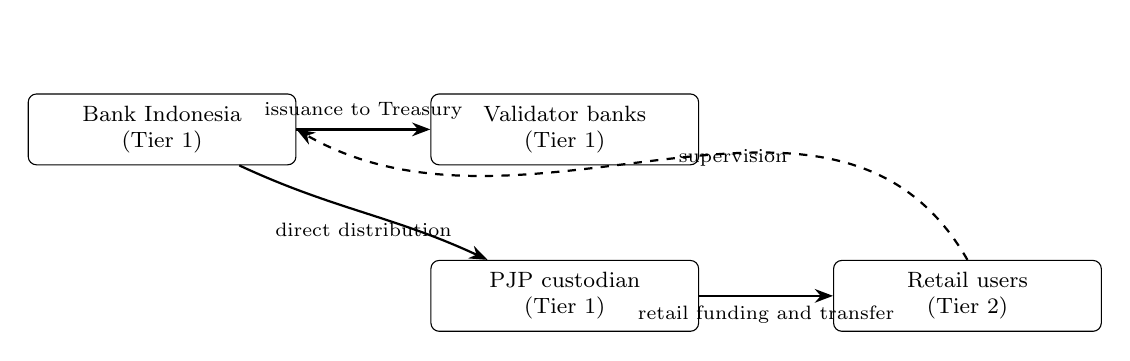
\begin{tikzpicture}[
  box/.style={draw=black, rounded corners=3pt, align=center,
    minimum width=3.4cm, minimum height=0.9cm, font=\footnotesize},
  ar/.style={-{Stealth}, thick}
]
\node[box] (bi) {Bank Indonesia\\ (Tier 1)};
\node[box, right=1.7cm of bi] (bank) {Validator banks\\ (Tier 1)};
\node[box, below=1.2cm of bank] (pjp) {PJP custodian\\ (Tier 1)};
\node[box, right=1.7cm of pjp] (retail) {Retail users\\ (Tier 2)};
\draw[ar] (bi) -- node[above, font=\scriptsize]{issuance to Treasury} (bank);
\draw[ar] (bi) to[out=-25,in=155] node[below, font=\scriptsize]{direct distribution} (pjp);
\draw[ar] (pjp) -- node[below, font=\scriptsize]{retail funding and transfer} (retail);
\draw[ar, dashed] (retail.north) to[out=120,in=-30]
  node[font=\scriptsize, right]{supervision} (bi.east);
\end{tikzpicture}%
}
\caption{Two-tier actor structure of the Digital Rupiah prototype. Bank
Indonesia issues Digital Rupiah into Treasury and distributes it directly to a
validator bank or PJP custodian, which serves retail users. Dashed flow denotes
supervisory visibility.}
\label{fig:twotier}
\end{figure}

\begin{table}[!t]
	\caption{Bank Indonesia Business Processes and Their Chaincode Realization}
	\label{tab:processes}
	\centering
	\scriptsize
	\setlength{\tabcolsep}{3.5pt}
	\begin{tabular}{ll>{\raggedright\arraybackslash}p{3.8cm}}
		\toprule
	\textbf{Process} & \textbf{Initiator} & \textbf{Chaincode transaction} \\
		\midrule
		Issuance       & Bank Indonesia & \texttt{Mint}, \texttt{RequestIssuance} \\
	Distribution   & Bank Indonesia & \texttt{DistributeToParticipant}        \\
		Wallet creation & Bank / PJP   & \texttt{CreateWallet}                  \\
		Payment        & Customer       & \texttt{Transfer}                        \\
		Redemption     & Participant    & \texttt{Burn}, \texttt{RequestRedemption} \\
		Supervision    & OJK / BI       & \texttt{GetReconciliationReport},
		\texttt{GetMetrics}, \texttt{GetSupervisionEvents}                         \\
		\bottomrule
	\end{tabular}

	\vspace{2pt}
	{\scriptsize The channel endorsement policy accepts an institutional MSP from
	Bank Indonesia, HimbaraBank, CommercialBank, or PJP; OJK is observer-only.}
\end{table}

The institutional tier contains Bank Indonesia, validator banks, and PJP
Custodians. These participants follow a lifecycle of submission, approval,
freezing, unfreezing, rejection, and offboarding. Bank Indonesia mints Digital
Rupiah only to the Treasury wallet, then distributes liquidity directly to an
active validator bank or PJP through \texttt{DistributeToParticipant}. Each
Custodian serves customers and merchants in the retail tier, where the shared
transfer path applies ownership, wallet-status, authorization, and balance
checks.

\section{System Architecture}
Fig.~\ref{fig:sysarch} shows the four-layer architecture: client, backend API,
off-chain store, and Fabric network. The web client calls a Go REST backend
built with Gorilla Mux. The backend authenticates requests with JWT and
role-based access control, stores account and authentication data in PostgreSQL,
and submits ledger transactions through the Fabric Gateway SDK.
Fig.~\ref{fig:netarch} details the permissioned network.

\begin{figure*}[!t]
	\centering
	\resizebox{\textwidth}{!}{%
		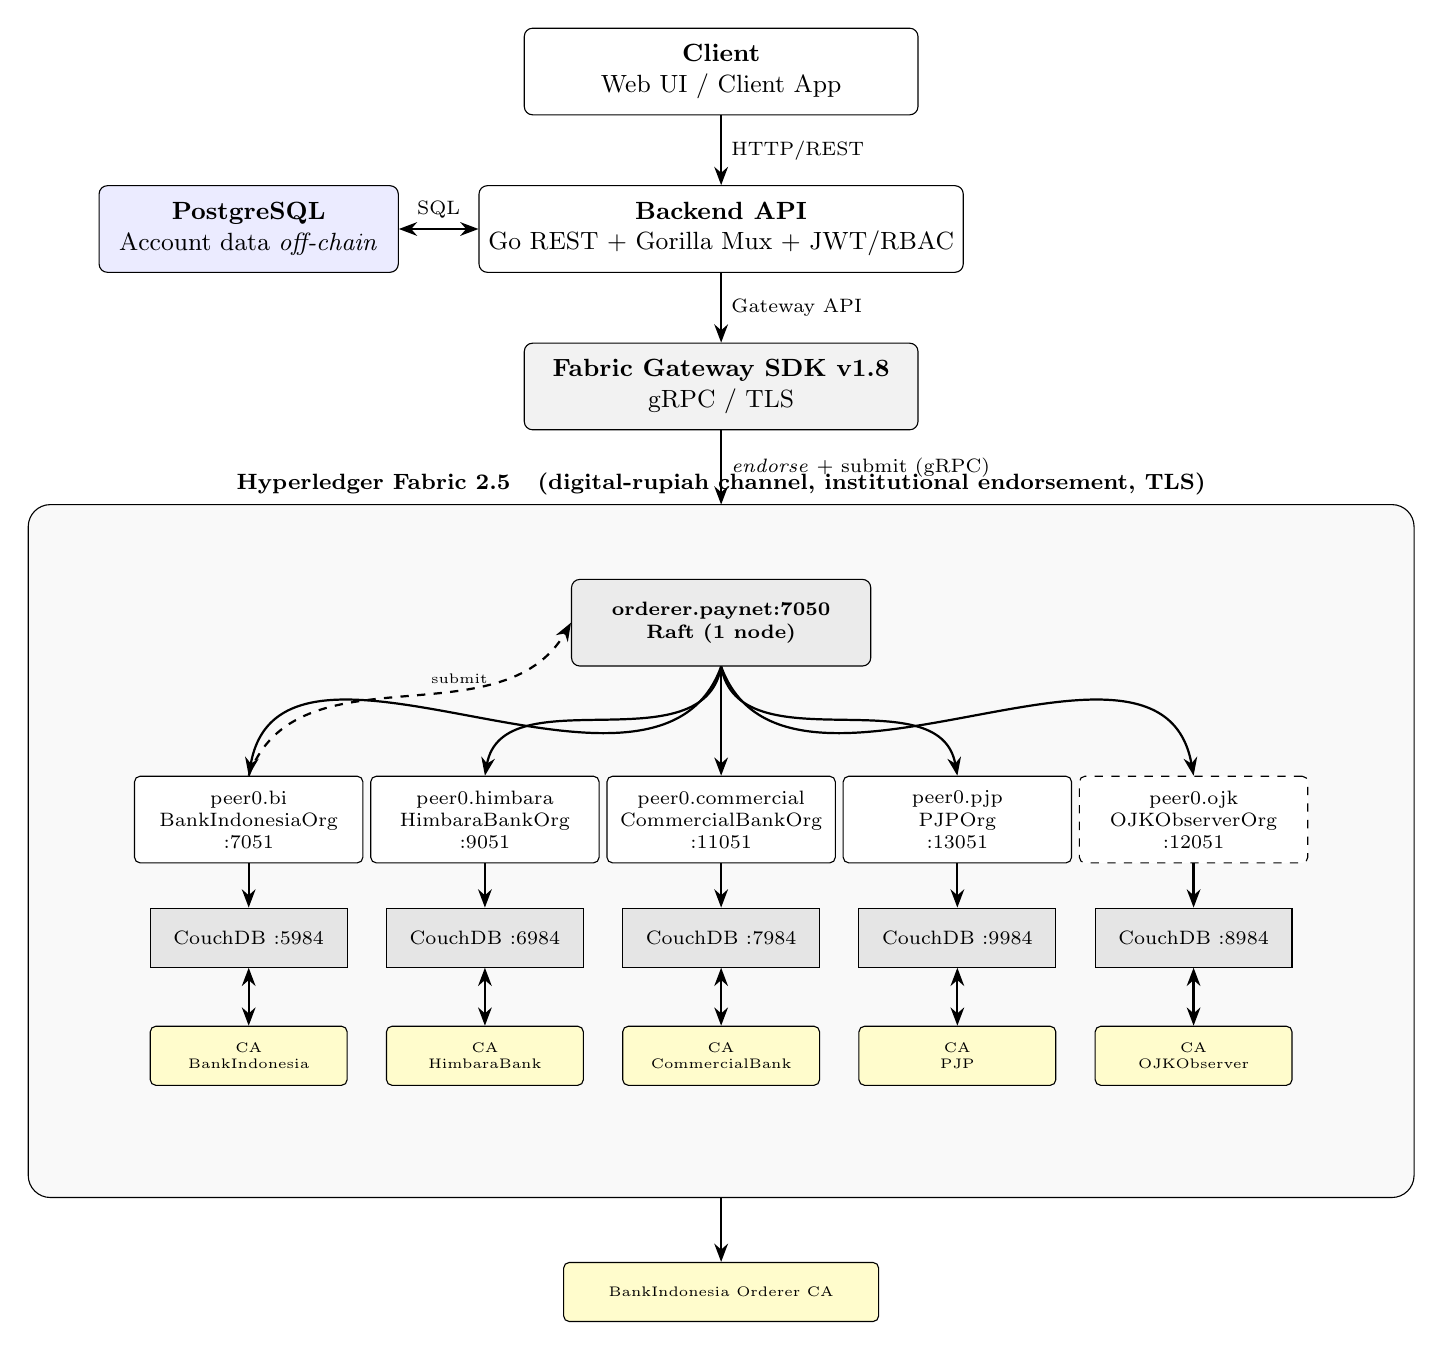
\begin{tikzpicture}[
				appbox/.style={draw=black, fill=white, rectangle, rounded corners=3pt,
						minimum width=5.0cm, minimum height=1.1cm, align=center, font=\small},
				gwbox/.style={draw=black, fill=black!5, rectangle, rounded corners=3pt,
						minimum width=5.0cm, minimum height=1.1cm, align=center, font=\small},
				pgbox/.style={draw=black, fill=blue!8, rectangle, rounded corners=3pt,
						minimum width=3.8cm, minimum height=1.1cm, align=center, font=\small},
				peer/.style={draw=black, fill=white, rectangle, rounded corners=2pt,
						minimum width=2.9cm, minimum height=1.1cm, align=center, font=\scriptsize},
				obsbox/.style={draw=black, dashed, fill=white, rectangle, rounded corners=2pt,
						minimum width=2.9cm, minimum height=1.1cm, align=center, font=\scriptsize},
				ordnode/.style={draw=black, fill=black!8, rectangle, rounded corners=3pt,
						minimum width=3.8cm, minimum height=1.1cm, align=center, font=\scriptsize\bfseries},
				cdb/.style={draw=black, fill=gray!20, rectangle,
						minimum width=2.5cm, minimum height=0.75cm, align=center, font=\scriptsize},
				cabox/.style={draw=black, fill=yellow!20, rectangle, rounded corners=2pt,
						minimum width=2.5cm, minimum height=0.75cm, align=center, font=\tiny},
				ar/.style={-{Stealth}, thick},
				bar/.style={{Stealth}-{Stealth}, thick},
				lbl/.style={font=\scriptsize, midway},
			]
			\node[appbox] (fe) at (6.0, 16.5) {\textbf{Client}\\Web UI / Client App};
			\node[appbox] (be) at (6.0, 14.5) {\textbf{Backend API}\\Go REST + Gorilla Mux + JWT/RBAC};
			\node[pgbox]  (pg) at (0.0, 14.5) {\textbf{PostgreSQL}\\Account data \textit{off-chain}};
			\node[gwbox]  (gw) at (6.0, 12.5) {\textbf{Fabric Gateway SDK v1.8}\\gRPC / TLS};
			\draw[ar]  (fe.south) -- (be.north)  node[lbl, right]{HTTP/REST};
			\draw[bar] (be.west)  -- (pg.east)   node[lbl, above]{SQL};
			\draw[ar]  (be.south) -- (gw.north)  node[lbl, right]{Gateway API};
			\fill[rounded corners=8pt, gray!5]  (-2.8, 2.2) rectangle (14.8, 11.0);
			\draw[rounded corners=8pt, black]   (-2.8, 2.2) rectangle (14.8, 11.0);
			\node[font=\footnotesize\bfseries, anchor=south] at (6.0, 11.0)
			{\textbf{Hyperledger Fabric 2.5}\quad
			(digital-rupiah channel, institutional endorsement, TLS)};
			\draw[ar] (gw.south) -- (6.0, 11.0)
			node[lbl, right]{\textit{endorse} + submit (gRPC)};
			\node[ordnode] (ord) at (6.0, 9.5) {orderer.paynet:7050\\Raft (1 node)};
			\node[peer]   (pbi)  at (0.0,  7.0) {peer0.bi\\BankIndonesiaOrg\\:7051};
			\node[peer]   (phim) at (3.0,  7.0) {peer0.himbara\\HimbaraBankOrg\\:9051};
			\node[peer]   (pcom) at (6.0,  7.0) {peer0.commercial\\CommercialBankOrg\\:11051};
			\node[peer]   (ppjp) at (9.0,  7.0) {peer0.pjp\\PJPOrg\\:13051};
			\node[obsbox] (pojk) at (12.0, 7.0) {peer0.ojk\\OJKObserverOrg\\:12051};
			\draw[ar] (ord.south) to[out=-110,in=80] (pbi.north);
			\draw[ar] (ord.south) to[out=-100,in=80] (phim.north);
			\draw[ar] (ord.south) -- (pcom.north);
			\draw[ar] (ord.south) to[out=-80,in=100]  (ppjp.north);
			\draw[ar] (ord.south) to[out=-70,in=100]  (pojk.north);
			\draw[ar, dashed] (pbi.north) to[out=70,in=-120]
			node[near end, left, font=\tiny]{submit} (ord.west);
			\node[cdb] (cbi)  at (0.0,  5.5) {CouchDB :5984};
			\node[cdb] (chim) at (3.0,  5.5) {CouchDB :6984};
			\node[cdb] (ccom) at (6.0,  5.5) {CouchDB :7984};
			\node[cdb] (cpjp) at (9.0,  5.5) {CouchDB :9984};
			\node[cdb] (cojk) at (12.0, 5.5) {CouchDB :8984};
			\draw[ar] (pbi)  -- (cbi);
			\draw[ar] (phim) -- (chim);
			\draw[ar] (pcom) -- (ccom);
			\draw[ar] (ppjp) -- (cpjp);
			\draw[ar] (pojk) -- (cojk);
			\node[cabox] (cabi)  at (0.0,  4.0) {CA\\BankIndonesia};
			\node[cabox] (cahim) at (3.0,  4.0) {CA\\HimbaraBank};
			\node[cabox] (cacom) at (6.0,  4.0) {CA\\CommercialBank};
			\node[cabox] (capjp) at (9.0,  4.0) {CA\\PJP};
			\node[cabox] (caojk) at (12.0, 4.0) {CA\\OJKObserver};
			\draw[bar] (cabi)  -- (cbi);
			\draw[bar] (cahim) -- (chim);
			\draw[bar] (cacom) -- (ccom);
			\draw[bar] (capjp) -- (cpjp);
			\draw[bar] (caojk) -- (cojk);
			\node[cabox, minimum width=4.0cm] (caord) at (6.0, 1.0) {BankIndonesia Orderer CA};
			\draw[ar] (6.0, 2.2) -- (caord.north);
		\end{tikzpicture}%
	}
	\caption{Full system architecture of the Digital Rupiah prototype: client
		layer, Go REST backend with JWT/RBAC, off-chain PostgreSQL store, Fabric
		Gateway SDK, and the Hyperledger Fabric 2.5 network of five peer
		organizations with CouchDB, a per-organization CA, and a Raft orderer.}
	\label{fig:sysarch}
\end{figure*}

\subsection{Network Topology}
The network runs five peer organizations on one application channel
(Fig.~\ref{fig:netarch}, Table~\ref{tab:topology}).
\emph{BankIndonesiaOrg} is the issuer; \emph{HimbaraBankOrg} (HIMBARA,
Indonesia's association of state-owned banks) and \emph{CommercialBankOrg} are
validator and distributor banks; \emph{PJPOrg} represents the payment service
provider; and \emph{OJKObserverOrg} is the supervisor (OJK, \emph{Otoritas Jasa
Keuangan}, the financial-services authority), which initiates no business
transactions and is excluded from chaincode approval. Each organization operates one
peer with a CouchDB world state and maintains its own certificate authority and
MSP for identity management. A single Raft orderer orders transactions; this
configuration provides ordering but not crash fault tolerance, which requires at
least three consenters. The
channel endorsement policy accepts one of the four institutional MSPs, while the
chaincode lifecycle policy requires Bank Indonesia and one institutional participant.

\begin{figure*}[!t]
	\centering
	\resizebox{\textwidth}{!}{%
		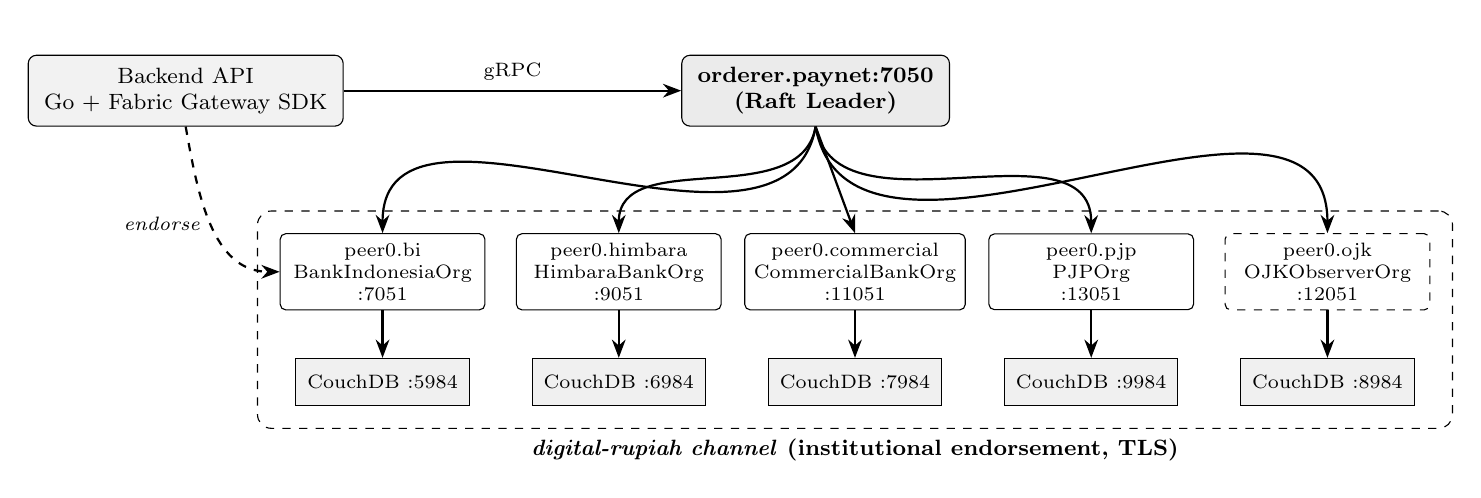
\begin{tikzpicture}[
				peer/.style={draw=black, fill=white, rectangle, rounded corners=2pt,
						minimum width=2.6cm, minimum height=0.9cm, align=center, font=\scriptsize},
				observer/.style={draw=black, dashed, fill=none, rectangle, rounded corners=2pt,
						minimum width=2.6cm, minimum height=0.9cm, align=center, font=\scriptsize},
				cdb/.style={draw=black, fill=gray!12, rectangle,
						minimum width=2.2cm, minimum height=0.6cm, align=center, font=\scriptsize},
				ordnode/.style={draw=black, fill=black!8, rectangle, rounded corners=3pt,
						minimum width=3.4cm, minimum height=0.9cm, align=center, font=\footnotesize\bfseries},
				backend/.style={draw=black, fill=black!5, rectangle, rounded corners=3pt,
						minimum width=4.0cm, minimum height=0.9cm, align=center, font=\footnotesize},
				chanbox/.style={draw=black, dashed, rounded corners=5pt, fill=none, inner sep=8pt},
				ar/.style={-{Stealth}, thick},
				gar/.style={-{Stealth}, thick, dashed},
				pathlabel/.style={font=\scriptsize, midway, align=center},
			]
			\node[backend] (be)  at (-2.5, 3.5) {Backend API\\Go + Fabric Gateway SDK};
			\node[ordnode] (ord) at ( 5.5, 3.5) {orderer.paynet:7050\\(Raft Leader)};
			\draw[ar] (be.east) -- node[pathlabel,above]{gRPC} (ord.west);
			\node[peer]     (pbi)  at ( 0.0, 1.2) {peer0.bi\\BankIndonesiaOrg\\:7051};
			\node[peer]     (phim) at ( 3.0, 1.2) {peer0.himbara\\HimbaraBankOrg\\:9051};
			\node[peer]     (pcom) at ( 6.0, 1.2) {peer0.commercial\\CommercialBankOrg\\:11051};
			\node[peer]     (ppjp) at ( 9.0, 1.2) {peer0.pjp\\PJPOrg\\:13051};
			\node[observer] (pojk) at (12.0, 1.2) {peer0.ojk\\OJKObserverOrg\\:12051};
			\draw[ar] (ord.south) to[out=-100,in=90] (pbi.north);
			\draw[ar] (ord.south) to[out=-100,in=90] (phim.north);
			\draw[ar] (ord.south) -- (pcom.north);
			\draw[ar] (ord.south) to[out=-80,in=90]  (ppjp.north);
			\draw[ar] (ord.south) to[out=-80,in=90]  (pojk.north);
			\draw[gar] (be.south) to[out=-80,in=180]
			node[pathlabel,left]{\textit{endorse}} (pbi.west);
			\node[cdb] (cbi)  at ( 0.0, -0.2) {CouchDB :5984};
			\node[cdb] (chim) at ( 3.0, -0.2) {CouchDB :6984};
			\node[cdb] (ccom) at ( 6.0, -0.2) {CouchDB :7984};
			\node[cdb] (cpjp) at ( 9.0, -0.2) {CouchDB :9984};
			\node[cdb] (cojk) at (12.0, -0.2) {CouchDB :8984};
			\draw[ar] (pbi)  -- (cbi);
			\draw[ar] (phim) -- (chim);
			\draw[ar] (pcom) -- (ccom);
			\draw[ar] (ppjp) -- (cpjp);
			\draw[ar] (pojk) -- (cojk);
			\node[chanbox, fit=(pbi)(phim)(pcom)(ppjp)(pojk)(cbi)(chim)(ccom)(cpjp)(cojk),
				label={[font=\footnotesize\bfseries]below:%
		\textit{digital-rupiah channel} (institutional endorsement, TLS)}] {};
		\end{tikzpicture}%
	}
	\caption{Hyperledger Fabric network topology: five peer organizations, each
		with a CouchDB world state, on a single channel under a Raft orderer; the
		Go backend endorses via the Fabric Gateway SDK.}
	\label{fig:netarch}
\end{figure*}

\begin{table}[!t]
	\caption{Network Topology of the Five-Organization Fabric Network}
	\label{tab:topology}
	\centering
	\scriptsize
	\setlength{\tabcolsep}{3.5pt}
	\begin{tabular}{lllr}
		\toprule
		\textbf{Organization} & \textbf{Role} & \textbf{Peer} & \textbf{CouchDB} \\
		\midrule
		BankIndonesiaOrg  & Issuer            & peer0.bi:7051         & :5984 \\
		HimbaraBankOrg    & Validator         & peer0.himbara:9051    & :6984 \\
		CommercialBankOrg & Validator         & peer0.commercial:11051 & :7984 \\
		PJPOrg            & Distributor       & peer0.pjp:13051       & :9984 \\
		OJKObserverOrg    & Supervisor        & peer0.ojk:12051       & :8984 \\
		\midrule
		\multicolumn{4}{l}{Ordering: orderer.paynet:7050 (single-node Raft); per-org CA;
		TLS enabled} \\
		\bottomrule
	\end{tabular}
\end{table}

\subsection{On-Chain and Off-Chain Data}
The Go chaincode in \texttt{digital\_rupiah.go} groups functions for
participants, wallets, issuance and redemption, retail transfers, and
supervision (Table~\ref{tab:funcs}). Account and authentication data remain in
the off-chain PostgreSQL store, while the ledger contains the wallet and
transaction state needed for settlement and oversight.

\begin{table}[!t]
	\caption{Chaincode Function Groups}
	\label{tab:funcs}
	\centering
	\footnotesize
	\setlength{\tabcolsep}{3.5pt}
	\begin{tabular}{l>{\raggedright\arraybackslash}p{6.0cm}}
		\toprule
		\textbf{Group} & \textbf{Representative functions} \\
		\midrule
		Participants & \texttt{SubmitParticipant}, \texttt{ApproveParticipant},
		\texttt{Freeze/Unfreeze}, \texttt{Offboard}                              \\
		Wallets      & \texttt{CreateWallet}, \texttt{CreateWholesaleWallet},
		\texttt{Freeze/UnfreezeWallet}                                           \\
		Issuance     & \texttt{Mint}, \texttt{RequestIssuance},
		\texttt{RequestIssuanceRtgs}                                             \\
		Redemption   & \texttt{Burn}, \texttt{RequestRedemption}                 \\
		Distribution & \texttt{DistributeToParticipant}                          \\
		Transfer     & \texttt{Transfer}                                         \\
		Supervision  & \texttt{GetReconciliationReport}, \texttt{GetMetrics},
		\texttt{GetSupervisionEvents}                                            \\
		\bottomrule
	\end{tabular}
\end{table}


A Go backend enforces role-based access control over six roles, summarized in
Table~\ref{tab:roles}, before any transaction reaches the chaincode.

\begin{table}[!t]
	\caption{Backend Roles and Representative Permissions}
	\label{tab:roles}
	\centering
	\footnotesize
	\setlength{\tabcolsep}{3.5pt}
	\begin{tabular}{l>{\raggedright\arraybackslash}p{5.7cm}}
		\toprule
		\textbf{Role} & \textbf{Representative permitted actions} \\
		\midrule
		Public          & Health check, login                         \\
		Authenticated   & View own profile, list wallets              \\
	Bank/PJP        & Create wallet, fund retail wallets         \\
		Bank Indonesia  & Issue, redeem liquidity, approve participant \\
		Merchant        & Initiate transfer, view balance             \\
		Supervisor      & Reconciliation, metrics, supervision events \\
		\bottomrule
	\end{tabular}
\end{table}

The two layers enforce different things, and the split matters for how the
prototype's guarantees should be read. The backend maps JWT roles to permitted
operations and restricts customers to their own wallets. The chaincode checks
the caller's organization, wallet status, transfer amount, and available
balance before it writes the state transition. Every endorsing peer re-evaluates
these rules independently, while the channel endorsement policy restricts
validation to institutional MSPs. The
single backend and PostgreSQL instance remain trust and availability
concentration points for this prototype.

\section{Protocol and Determinism}
\label{sec:proto}
The transfer path applies explicit authorization and balance checks during
endorsement. We formalize these checks and examine their behavior under
concurrent transactions.

\subsection{Transfer-Validity Rules}
For a transfer of amount $a$ from sender $s$ to receiver $r$, the chaincode
admits the transfer only if every one of the following checks passes:
\begin{itemize}
\item the caller's organization and wallet ownership satisfy the authorization
      rules;
\item neither the sender's nor the receiver's wallet is frozen;
\item $a>0$ and the required business reference is present;
\item the sender has enough balance to cover $a$; and
\item the sender and receiver wallet records can be updated atomically.
\end{itemize}
If any check fails, the transfer is rejected. A successful transfer decreases
the sender balance, increases the receiver balance, records the transaction,
and emits the supervision event used by the read-only observer path. Treasury
distribution accepts only active validator-bank or PJP custodians, and a PJP
cannot call issuance directly.

\subsection{Determinism and Double-Spend Safety}
Every endorsing peer evaluates the authorization and transfer rules against the
same transaction arguments and wallet records. The state transition does not
depend on a peer-local clock or on a peer-local cache. Each successful transfer
updates the sender and receiver records in one transaction, so every endorser
evaluates the same balance transition before validation.

Double-spend safety follows from Fabric's multi-version concurrency control
(MVCC). An endorsement reads the current version of each wallet record, and
Fabric commits the transaction only if those versions remain unchanged through
ordering and validation. Two concurrent transfers from the same wallet may
endorse against the same record and version, but only the first ordered
transaction commits. The second fails MVCC validation after the first update.
Because the balance records are the keys in the read set, one version check
covers the state used by the transfer and prevents a stale balance update.

\begin{figure}[!t]
\centering
\begin{algorithmic}[1]
\STATE \textbf{function} \textsc{Transfer}(sender, receiver, amount)
\IF{caller unauthorized \textbf{or} either wallet is frozen}
\RETURN \textsc{reject}
\ENDIF
\IF{amount $\le 0$ \textbf{or} reference is missing}
\RETURN \textsc{reject}
\ENDIF
\IF{sender.balance $<$ amount}
\RETURN \textsc{reject}
\ENDIF
\STATE sender.balance $\leftarrow$ sender.balance $-$ amount
\STATE receiver.balance $\leftarrow$ receiver.balance $+$ amount
\STATE append transaction history and emit supervision event
\STATE \textbf{PutState} (validated by Fabric MVCC)
\RETURN \textsc{commit}
\end{algorithmic}
\caption{Authorized, atomic, and double-spend-safe transfer executed by the
chaincode. Fabric MVCC validates the wallet versions before commit.}
\label{alg:transfer}
\end{figure}


\section{Performance Evaluation}
\label{sec:eval}

\subsection{Methodology}
We evaluate the final prototype with Hyperledger Caliper 0.6.0 on a clean
ledger for each profile. The combined manifest
\texttt{20260909-final-evidence-manifest.json} records suite seed 20260909
(profile ordering); the transfer configurations retain workload seed 20260725.
It also records chaincode \texttt{digital-rupiah} version 3.0 sequence 1, runtime versions,
input hashes, result hashes, and the single-host topology. The testbed has five
peer organizations, one peer per organization, one Raft orderer, and one
CouchDB instance per peer.

\begin{table}[!t]
\caption{Final testbed configuration}
\label{tab:testbed-final}
\centering
\scriptsize
\begin{tabular}{l>{\raggedright\arraybackslash}p{5.2cm}}
\toprule
\textbf{Component} & \textbf{Specification} \\
\midrule
Processor & Intel Core i7-7700HQ, 4 cores, 8 threads, 2.80 GHz \\
Memory & 15.52 GiB \\
Runtime & Node.js 22.23.2, npm 10.9.1, Docker 27.5.1 \\
Fabric / CouchDB & 2.5 / 3.2 \\
Caliper & 0.6.0 \\
Chaincode & \texttt{digital-rupiah} v3.0, sequence 1 \\
Ordering & Single-node Raft; batch timeout 2 s; maximum 10 messages \\
Endorsement & One institutional MSP: BI, HimbaraBank, CommercialBank, or PJP \\
\bottomrule
\end{tabular}
\end{table}

The transfer profiles use 70\% customer-to-customer transfers, 25\%
customer-to-merchant transfers, and 5\% wallet reads. Each profile warms the
network for 30 seconds at 10 TPS, then measures 120-second rounds at 30 and
60 TPS. The one-, two-, and four-worker profiles use the populations and
transaction slots specified in their individual configuration files. Sender
wallets receive a larger initial balance than receiver wallets, so valid
traffic does not begin with a receiver at its maximum balance. Caliper records
successful and failed submissions, completion throughput, and latency.

\begin{table}[!t]
\caption{Final transfer-profile results}
\label{tab:results-final}
\centering
\scriptsize
\setlength{\tabcolsep}{1.8pt}
\begin{tabular}{@{}llrrrrrr@{}}
\toprule
\textbf{Workers} & \textbf{Load} & \textbf{Succ.} & \textbf{Fail} &
\textbf{Success} & \textbf{Send} & \textbf{Throughput} & \textbf{Avg.} \\
& & & & \textbf{(\%)} & \textbf{(TPS)} & \textbf{(TPS)} & \textbf{lat. (s)} \\
\midrule
1 & 30 TPS & 3,105 & 496 & 86.23 & 30.0 & 29.1 & 0.71 \\
1 & 60 TPS & 898 & 6,300 & 12.48 & 60.0 & 56.3 & 6.36 \\
2 & 30 TPS & 3,602 & 0 & 100.00 & 30.0 & 29.5 & 0.40 \\
2 & 60 TPS & 874 & 6,327 & 12.14 & 60.0 & 57.2 & 6.48 \\
4 & 30 TPS & 3,486 & 118 & 96.73 & 30.0 & 29.5 & 0.76 \\
4 & 60 TPS & 868 & 6,336 & 12.05 & 60.0 & 57.3 & 6.47 \\
\bottomrule
\end{tabular}
\end{table}

All warmup rounds completed without failure. At 30 TPS, completion throughput
was 29.1--29.5 TPS and success rate was 86.23--100.00\%. At 60 TPS, completion
throughput was 56.3--57.3 TPS while success rate was 12.05--12.48\%. Completion
throughput includes failed submissions, so it is not successful throughput.

\begin{table}[!t]
\caption{Failure diagnostics in final transfer profiles}
\label{tab:failure-diagnostics-final}
\centering
\scriptsize
\begin{tabular}{@{}lrrr@{}}
\toprule
\textbf{Profile} & \textbf{Status 11} & \textbf{Gateway limit} & \textbf{Total} \\
\midrule
1 worker & 5,332 & 1,464 & 6,796 \\
2 workers & 4,919 & 1,408 & 6,327 \\
4 workers & 5,121 & 1,333 & 6,454 \\
Five repetitions & 11,878 & 3,191 & 15,069 \\
\bottomrule
\end{tabular}
\end{table}

The final transfer logs classify every failed submission as Fabric status 11 or
the gateway message \texttt{too many requests for /gateway.Gateway}. Status 11
is the Fabric validation code for an MVCC read conflict: a transaction read a
wallet version that changed before commit. The gateway message identifies
client-path concurrency pressure. The logs contain no insufficient-balance or
transport failure in these final transfer profiles.

\begin{table}[!t]
\caption{Five repetitions at an offered load of 60 TPS}
\label{tab:repeat-final}
\centering
\scriptsize
\begin{tabular}{@{}lrrrrr@{}}
\toprule
\textbf{Round} & \textbf{Succ.} & \textbf{Fail} & \textbf{Success (\%)} &
\textbf{Throughput (TPS)} & \textbf{Avg. lat. (s)} \\
\midrule
1 & 895 & 2,707 & 24.85 & 57.7 & 3.23 \\
2 & 403 & 3,199 & 11.19 & 54.9 & 6.93 \\
3 & 598 & 3,004 & 16.60 & 54.8 & 4.93 \\
4 & 448 & 3,154 & 12.44 & 52.7 & 6.39 \\
5 & 597 & 3,005 & 16.57 & 54.1 & 4.50 \\
\midrule
Mean & 588.2 & 3,013.8 & 16.33 & 54.8 & 5.20 \\
\bottomrule
\end{tabular}
\end{table}

Five repetitions on one clean ledger produced a mean completion throughput of
54.8 TPS and a mean success rate of 16.33\%. The success-rate range was
11.19--24.85\%, and mean latency ranged from 3.23 to 6.93 s. These values
describe variation in the reported local configuration.

\begin{table}[!t]
\caption{Functional Caliper profiles}
\label{tab:functionality-final}
\centering
\scriptsize
\begin{tabular}{@{}lrrrr@{}}
\toprule
\textbf{Profile} & \textbf{Succ.} & \textbf{Fail} & \textbf{Throughput (TPS)} &
\textbf{Avg. lat. (s)} \\
\midrule
KYC onboarding & 48 & 0 & 4.3 & 0.74 \\
Monetary operations & 40 & 0 & 19.4 & 0.33 \\
Supervision reads & 40 & 0 & 30.6 & 0.03 \\
Administrative policy & 40 & 0 & 5.1 & 1.05 \\
\bottomrule
\end{tabular}
\end{table}

The four functional profiles completed all 168 transactions without failure.
They verify onboarding, monetary operations, read-only supervision, and policy
updates at their configured rates. Their throughputs are not combined with the
transfer sweep because the functions and read-write patterns differ.

\begin{table}[!t]
\caption{Semantic conformance profiles}
\label{tab:conformance-final}
\centering
\scriptsize
\begin{tabular}{@{}lrrp{4.6cm}@{}}
\toprule
\textbf{Profile} & \textbf{Succ.} & \textbf{Fail} & \textbf{Oracle result} \\
\midrule
Authorization & 2 & 1 & PASS; one expected custodian-mismatch rejection. \\
Boundary & 4 & 4 & PASS; 8/8 cases, zero mismatches, zero infrastructure errors. \\
Negative path & 0 & 7 & PASS; 7/7 expected rejection rules enforced. \\
Aggregate overspend & 10 & 190 & PASS; final sender balance Rp40,000. \\
\bottomrule
\end{tabular}
\end{table}

The failed counts in these semantic profiles represent expected policy
rejections. The aggregate-overspend workload requested Rp200,000 from an
initial Rp50,000 sender balance. Ten transfers committed and 190 were rejected;
the final balance remained Rp40,000. These observations support the tested
authorization and balance invariants, but do not constitute a formal security
proof.

\begin{table}[!t]
\caption{Maximum monitored resource usage}
\label{tab:resources-final}
\centering
\scriptsize
\begin{tabular}{@{}lrr@{}}
\toprule
\textbf{Profile} & \textbf{CPU max. (\%)} & \textbf{Memory max. (MB)} \\
\midrule
Transfer, 1 worker & 2.35 & 163 \\
Transfer, 2 workers & 2.74 & 166 \\
Transfer, 4 workers & 2.69 & 163 \\
Five peak repetitions & 2.53 & 170 \\
\bottomrule
\end{tabular}
\end{table}

No monitored container approached the host CPU or memory capacity. The
observed drop in success at 60 TPS therefore cannot be attributed to simple
resource exhaustion alone; the logs show state conflicts and gateway
concurrency pressure. The evidence supports the architecture and policy
controls, then bounds their observed behavior under the tested local loads.

\section{Limitations and Future Work}
\label{sec:limits}
The evaluation uses a single host with one peer per organization and no
geographic distribution or network latency. Its Caliper results therefore apply
only to the reported configuration and do not estimate national-scale
performance. Each transfer profile uses a clean ledger and a fixed seeded
population, while the final sweep varies one, two, and four workers. A
distributed deployment and a graded-skew contention workload would be needed to
characterize other operating conditions.

The shared Fabric channel does not provide transaction privacy, and the
prototype does not use private data collections or privacy-preserving
cryptography. The single orderer provides ordering but does not tolerate its
own failure. The prototype also omits offline payment and leaves connections to
domestic infrastructure such as BI-RTGS and BI-FAST as stubs.

The authorization and aggregate-overspend profiles cover the tested paths only.
They do not establish formal security, production readiness, or
cross-machine reproducibility. Future work should repeat the protocol on
distributed hosts, instrument endorsement and commit phases, expand the
contention workload, and evaluate privacy, offline payment, and
interoperability.


\section{Conclusion}
This paper implements Bank Indonesia's digital money business processes in a
two-tier Digital Rupiah prototype on a five-organization Hyperledger Fabric
network. The chaincode integrates hierarchical issuance and distribution,
retail transfers, organization-aware authorization, and supervisor-facing
reconciliation.

The transfer protocol combines explicit wallet-state checks with Fabric MVCC.
The final Caliper sweep reports 29.1--29.5 TPS completion throughput at a
30 TPS offered load with an 86.23--100.00\% success rate. At 60 TPS, completion
throughput is 56.3--57.3 TPS and success rate is 12.05--12.48\%. Five peak
repetitions average 54.8 TPS completion throughput and 16.33\% success. The
functional profiles complete 168 of 168 transactions, and the authorization,
boundary, negative-path, and aggregate-overspend oracles pass their expected
checks. These results provide a local, auditable baseline for retail Digital
Rupiah experiments, not a production-capacity claim.


\section*{Artifact Availability}
The chaincode, the five-organization network definition, the Go backend, and the
Hyperledger Caliper workloads and benchmark configurations used in this paper are
available at \url{https://github.com/mfachrizalg/bi-coin}.

\bibliographystyle{IEEEtran}
\bibliography{references}

\end{document}
